\documentclass[aspectratio=169,t,xcolor=table]{beamer}
\usepackage[utf8]{inputenc}
\usepackage[brazil]{babel}
\usepackage{booktabs,tabularx,listings}
\usetheme{Ufg}
\ifXeTeX
  \renewcommand{\encodingdefault}{TU}
  \fontencoding{TU}\selectfont
\fi
\usetikzlibrary{arrows.meta,positioning,fit,backgrounds,babel}

\setPrimaryColor{UFGBlue}
\setLogos{lib/logos/INF-compact-white.png}{lib/logos/INF-compact-white.png}
\setbeamertemplate{note page}[plain]
\setbeameroption{hide notes}
\newcolumntype{Y}{>{\raggedright\arraybackslash}X}
\tikzset{
  component/.style={draw=UFGBlue!85!black,fill=Ocean!23,text=DarkGray,
    rounded corners=3pt,align=center,minimum height=10mm,inner sep=3pt,font=\small},
  output/.style={component,draw=DarkGreen!85!black,fill=LightGreen!16},
  flow/.style={-{Stealth[length=2mm]},draw=UFGBlue!85!black,thick},
  edge label/.style={inner sep=1pt,text=DarkGray,fill=white,font=\scriptsize,align=center}
}

\title[TowerAI]{TowerAI}
\subtitle{Registro de reuniões com contexto e processamento local}
\author[Pequi Ubíquo]{Thiago Nascente \and Samuel Machado \and Moisés Protázio \and Vinícius Benevides}
\institute[INF/UFG]{Instituto de Informática da UFG\\Software para Sistemas Ubíquos (INF0483)}
\date{Marco 4 · 2026}

\begin{document}
\frame[noframenumbering]{\titlepage}
\note{0:20. Apresentar o grupo. A versão do painel demonstrada é 4.1.4 e o APK da evidência é 4.0.1.}

\setLayout{vertical}
\begin{frame}{O que é o TowerAI}
  \begin{block}{Registro de reuniões em uma sala}
    Um participante arma o microfone do Android. O notebook usa o som e a presença estimada pela webcam para decidir quando gravar.
  \end{block}
  \vspace{0.65em}
  \begin{itemize}
    \item Ao encerrar, o notebook transcreve o áudio e gera uma ata com decisões e tarefas.
    \item A equipe revisa a reunião no Android e exporta o histórico em PDF com o áudio anexo no servidor.
    \item A captura e o processamento funcionam na LAN com os modelos já instalados.
  \end{itemize}
\end{frame}
\note{0:45. Motivar com a dificuldade de acompanhar a conversa e recuperar responsáveis e prazos. Explicar que o usuário decide quando armar o microfone.}

\begin{frame}{Evolução entre os marcos}
  \vspace{0.6em}
  \small
  \begin{tabularx}{\textwidth}{@{}lYY@{}}
    \toprule
    \textbf{Marco} & \textbf{Entrega} & \textbf{Resultado para o projeto} \\ \midrule
    1 & Cenário multimodal e modelagem de contexto. & Processamento na borda e percepção da sala. \\
    \addlinespace
    2 & ESP32/Wokwi, MQTT e consumidor Python. & ACK, reenvio e decisão com estado. \\
    \addlinespace
    3 & HiveMQ com TLS, contas e permissões por tópico. & Identidade, canal protegido e resumo da sessão. \\
    \addlinespace
    4 & Android, webcam, API HTTPS e ata persistente. & Fluxo completo com captura, revisão e PDF. \\
    \bottomrule
  \end{tabularx}
\end{frame}
\note{0:55. O Marco 2 transmitia mudanças de estado. O Marco 4 envia amostras de áudio para transcrição e mantém as garantias de confirmação e autoria. A API HTTPS toma o lugar do broker nesta versão.}

\setLayout{horizontal}
\begin{frame}{Arquitetura do Marco 4}
  \centering
  \begin{tikzpicture}[x=1cm,y=1cm]
    \node[output,text width=21mm] (android) at (-5.35,0.5) {\textbf{Android}\\Kotlin / Compose};
    \node[component,text width=21mm] (camera) at (-0.75,2.2) {\textbf{Webcam}\\OpenCV / YOLOX-S};
    \node[component,text width=21mm] (api) at (-0.75,0.5) {\textbf{API Python}\\Identidade e ACK};
    \node[component,text width=22mm] (rule) at (3.2,0.5) {\textbf{Regra da sala}\\Estado e fila};
    \node[component,text width=24mm] (models) at (3.2,2.2) {\textbf{Inferência}\\Whisper / Qwen};
    \node[component,text width=23mm] (db) at (3.2,-1.05) {\textbf{SQLite}\\Dados e resultados};
    \node[output,text width=21mm] (desktop) at (-0.75,-1.05) {\textbf{Tkinter}\\PDF com WAV};
    \draw[flow,<->] (android) -- node[edge label,above] {LAN: HTTPS} node[edge label,below] {Áudio e histórico} (api);
    \draw[flow] (camera) -- node[edge label,left] {HTTPS (CLI)} (api);
    \draw[flow,dashed] (camera.south east) -- node[edge label,above,sloped] {Local (painel)} (rule.north west);
    \draw[flow] (api) -- (rule);
    \draw[flow,<->] (rule) -- (models);
    \draw[flow,<->] (rule) -- (db);
    \draw[flow] (db) -- (desktop);
    \begin{scope}[on background layer]
      \node[draw=UFGBlue!50,dashed,rounded corners=4pt,fit=(camera)(api)(rule)(models)(db)(desktop),
        inner xsep=4mm,inner ysep=2mm,label={[font=\scriptsize,text=UFGBlue!85!black]above:Notebook}] {};
    \end{scope}
  \end{tikzpicture}
\end{frame}
\note{1:00. Explicar por que a inferência e o estado ficam no notebook. A webcam atua como segundo produtor. Em linha de comando, publica com credencial própria por HTTPS. No painel, publica localmente com uma identidade interna. O llama.cpp recebe texto em loopback.}

\setLayout{horizontal}
\begin{frame}{Modo de uso}
  \begin{columns}[c,onlytextwidth]
    \column{.73\textwidth}
    \begin{enumerate}
      \item \textbf{Notebook.} Gere o certificado, cadastre o microfone e ligue o servidor.
      \item \textbf{Android.} Importe a CA, informe a origem HTTPS e a credencial. Conecte e arme o microfone.
      \item \textbf{Reunião.} Acompanhe o estado e encerre pelo app ou pelo silêncio.
      \item \textbf{Histórico.} Revise a reunião no app. Na aba \textbf{Histórico} do servidor, exporte o PDF.
    \end{enumerate}
    \column{.25\textwidth}
    \centering
    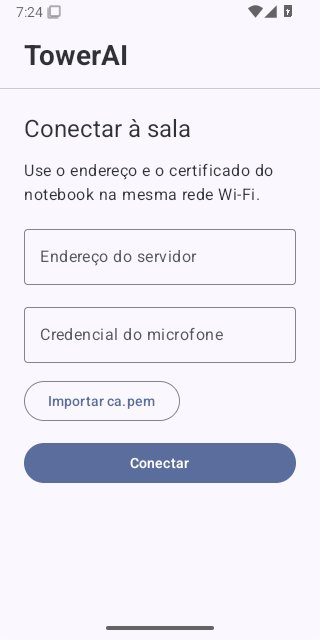
\includegraphics[height=4.3cm]{figs/towerai-android.jpg}
  \end{columns}
\end{frame}
\note{0:55. Mostrar o APK preparado, sem exibir a credencial. A configuração do painel também inclui escolher a webcam e preparar os modelos.}

\setLayout{horizontal}
\begin{frame}{Contexto, estado e validade}
  \centering
  \begin{tikzpicture}[node distance=11mm]
    \node[component,text width=22mm] (waiting) {Aguardando};
    \node[output,text width=22mm,right=of waiting] (recording) {Aberta};
    \node[component,text width=22mm,right=of recording] (ending) {Encerrando};
    \node[component,text width=22mm,right=of ending] (closed) {Fechada};
    \draw[flow] (waiting) -- node[edge label,above] {3 blocos} (recording);
    \draw[flow] (recording) -- node[edge label,above] {Silêncio} (ending);
    \draw[flow] (ending) -- node[edge label,above] {10 blocos} (closed);
  \end{tikzpicture}
  \vspace{0.75em}
  \begin{itemize}
    \item Abertura com 3 s de áudio a pelo menos $-42$ dBFS e presença positiva ou desconhecida.
    \item Presença válida igual a zero bloqueia a abertura. A leitura expira em 15 s.
    \item Um bloco sonoro interrompe o encerramento. A parada manual fecha a captura.
  \end{itemize}
\end{frame}
\note{0:55. Demonstrar primeiro presença zero e depois uma leitura positiva. Se a câmera estiver indisponível, a presença desconhecida permite abertura com marca de incerteza. A suspensão por falha aparece no próximo bloco da apresentação.}

\setLayout{vertical}
\begin{frame}{Comunicação entre produtores e API}
  \begin{itemize}
    \item \textbf{Microfone.} PCM16 mono a 16 kHz, em blocos de 1 s numerados e datados pela referência do servidor.
    \item \textbf{Webcam.} Contagem, horário e identificador. A CLI envia JSON por HTTPS. O painel publica no próprio processo.
    \item \textbf{ACK.} O SQLite confirma o efeito antes da resposta. Uma repetição idêntica recebe ACK de duplicado.
    \item \textbf{Conflito.} Saltos de sequência ou reuso com bytes diferentes recebem HTTP 409.
  \end{itemize}
\end{frame}
\note{0:50. O Android combina o Date da API com relógio monotônico. A fila em memória preserva sequência e horário. O detalhe está no contrato v1 do artigo.}

\begin{frame}{Autenticação e autorização}
  \begin{itemize}
    \item \textbf{Serviço.} HTTPS com TLS 1.2 ou superior. O app valida a CA local e confere o endereço no SAN.
    \item \textbf{Produtor.} Token Bearer individual, associado no servidor a identificador, papel e sala.
    \item \textbf{Permissões.} A webcam publica presença. O microfone lê o histórico da sala, e só o dono controla sua captura.
    \item \textbf{Operação.} Segredos ficam na instalação. O modelo de texto recebe dados em loopback.
  \end{itemize}
\end{frame}
\note{0:55. Separar verificação da identidade do notebook e verificação da identidade do produtor. Usar saídas registradas de CA desconhecida, SAN incorreto e recusa por papel. O notebook e sua conta local fazem parte do modelo de confiança.}

\setLayout{horizontal}
\begin{frame}{Processamento e persistência}
  \centering
  \begin{tikzpicture}[node distance=5mm]
    \node[component,text width=22mm] (pcm) {Áudio aceito\\no SQLite};
    \node[component,text width=22mm,right=of pcm] (stt) {Faster Whisper\\Large v3 / Turbo};
    \node[component,text width=22mm,right=of stt] (llm) {Qwen2.5\\via llama.cpp};
    \node[output,text width=22mm,right=of llm] (ata) {Ata em JSON\\no SQLite};
    \draw[flow] (pcm) -- (stt); \draw[flow] (stt) -- (llm); \draw[flow] (llm) -- (ata);
  \end{tikzpicture}
  \vspace{0.65em}
  \begin{itemize}
    \item Os segmentos são salvos antes da ata. Se a geração falhar, a fila reutiliza a transcrição.
    \item O histórico sobrevive ao reinício e reabre no Android.
    \item Mesmo com a API parada, o painel exporta ata e transcrição em PDF e anexa a gravação salva em WAV.
  \end{itemize}
\end{frame}
\note{1:00. Encerrar uma captura, abrir uma ata pronta, reiniciar a API e recuperar o mesmo registro. Usar a aba Histórico no servidor para exportar o PDF. Mostrar a ata, a transcrição e o WAV no painel de anexos do leitor de PDF.}

\setLayout{vertical}
\begin{frame}{Falha e recuperação da captura}
  \begin{enumerate}
    \item Após \textbf{6 s sem áudio fresco}, a reunião fica suspensa e recebe a marca de captura incompleta.
    \item Um bloco antigo pode completar o histórico. Um bloco fresco retoma a avaliação ao vivo.
    \item Após \textbf{mais 60 s de interrupção}, o servidor fecha a reunião como incompleta.
  \end{enumerate}
  \vspace{0.45em}
  \begin{block}{Demonstração}
    Uma queda breve do Wi-Fi interrompe o envio. Após reconectar, o Android entrega a fila sem duplicar os blocos já confirmados.
  \end{block}
\end{frame}
\note{1:10. Desativar o Wi-Fi por cerca de oito segundos durante a gravação. Mostrar o efeito observado na qualidade da captura após reconectar. Ter o resultado do teste como apoio.}

\begin{frame}{O que os testes comprovaram}
  \vspace{0.4em}
  \small
  \begin{tabularx}{\textwidth}{@{}lY@{}}
    \toprule
    \textbf{Verificação} & \textbf{Resultado observado} \\ \midrule
    API HTTPS e estado & Sala vazia bloqueou a abertura. Um bloco fresco retomou a captura suspensa. \\
    \addlinespace
    Segurança & CA ou SAN incompatível falhou. A API recusou operações fora do papel ou da sala. \\
    \addlinespace
    Histórico & ID, ata e transcrição sobreviveram ao reinício. O WAV anexo preservou o áudio recebido. \\
    \addlinespace
    APK Android & Três testes JVM e dois instrumentados aprovados no registro do Android 4.0.1. \\
    \bottomrule
  \end{tabularx}
  \vspace{0.6em}

  {\small 20 testes Python aprovados no servidor 4.1.4. Comandos e evidências no guia de verificação.}
\end{frame}
\note{0:55. Distinguir emulador Android, teste automatizado com sinais injetados e ensaio de modelos. Mostrar o log de teste ou executar a suíte Python.}

\begin{frame}{Resultados do ensaio de inferência}
  \vspace{0.35em}
  \small
  \begin{tabularx}{\textwidth}{@{}lrrY@{}}
    \toprule
    \textbf{Whisper} & \textbf{Qwen} & \textbf{Fluxo} & \textbf{Resultado da ata} \\ \midrule
    Large v3 Turbo & 7B & 29,86 s & Decisão futura e duas ações corretas. \\
    \addlinespace
    Large v3 & 7B & 47,88 s & Mesma decisão e atribuições. \\
    \addlinespace
    Large v3 Turbo & 1.5B & 16,32 s & Duas ações corretas. Descreveu a decisão futura como concluída. \\
    \bottomrule
  \end{tabularx}
  \vspace{0.65em}

  {\small WAV sintético de 17 s com presença injetada. Whisper em CUDA, Qwen em CPU. O tempo inclui entrega, processamento, reinício e consulta.}
\end{frame}
\note{0:55. Comparar as configurações mantendo um modelo de cada vez. Explicar que o pacote padrão em CPU usa Qwen 1.5B. A leitura humana é necessária para conferir sentido e prazos. Fonte: os três arquivos ensaio-*.json descritos no artigo.}

\begin{frame}{Implantação e reprodução}
  \begin{itemize}
    \item \textbf{Distribuição.} APK Android e servidor 4.1.4 para Windows x64 e Ubuntu amd64.
    \item \textbf{Preparação.} Modelos locais, rede da sala e CA importada. Os guias documentam dependências, armazenamento e ordem de execução.
    \item \textbf{Repositório.} Código, diagrama, contrato v1, comandos de teste e artigo técnico.
  \end{itemize}
\end{frame}
\note{0:40. Mostrar o README e os guias de implantação. Antes da apresentação, registrar o commit demonstrado e o hash do APK. Contribuições individuais e feedback do Marco 3 devem ser relatados pelo grupo com base nos registros efetivos.}

\begin{frame}{Limites da avaliação}
  \begin{itemize}
    \item Iluminação, oclusão e enquadramento afetam a estimativa da webcam. Energia sonora aproxima atividade de fala.
    \item Uma interrupção longa ou o encerramento do app pode perder blocos ainda sem confirmação.
    \item A avaliação com fala sintética não mede reuniões espontâneas, consumo de bateria ou latência sob carga.
    \item A equipe deve conferir a ata com a transcrição antes de distribuí-la.
  \end{itemize}
\end{frame}
\note{1:00. Fechar com o que o ensaio sustenta e com os limites de privacidade do histórico e do PDF. Reservar a fala final para os quatro integrantes explicarem sua participação real e relatarem o atendimento ao feedback com a evidência correspondente.}

\end{document}
